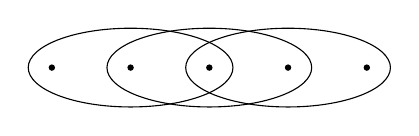
\begin{tikzpicture}
\draw (0,0) node[draw,shape=circle, fill=black, scale=.2]{}
	  (1,0) node[draw,shape=circle, fill=black, scale=.2]{}
	  (2,0) node[draw,shape=circle, fill=black, scale=.2]{}
      (3,0) node[draw,shape=circle, fill=black, scale=.2]{}
	  (4,0) node[draw,shape=circle, fill=black, scale=.2]{};
\draw (1,0) ellipse (1.3 and .5);
\draw (2,0) ellipse (1.3 and .5);
\draw (3,0) ellipse (1.3 and .5);
\end{tikzpicture}
\hspace{1cm}
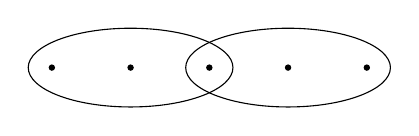
\begin{tikzpicture}
\draw (0,0) node[draw,shape=circle, fill=black, scale=.2]{}
(1,0) node[draw,shape=circle, fill=black, scale=.2]{}
(2,0) node[draw,shape=circle, fill=black, scale=.2]{}
(3,0) node[draw,shape=circle, fill=black, scale=.2]{}
(4,0) node[draw,shape=circle, fill=black, scale=.2]{};
\draw (1,0) ellipse (1.3 and .5);
\draw (3,0) ellipse (1.3 and .5);
\end{tikzpicture}